% =====================================================================
%  The periodic-equilibrium solver: origin, calculation, validation, C++.
%  A detailed defence of the method (old brute-force spin-up vs. the new
%  flux-anchored solver). Self-contained for Overleaf: upload this folder
%  (justification.tex + figures/).  Compile:  latexmk -pdf justification.tex
% =====================================================================
\documentclass[11pt]{article}

\usepackage[a4paper,margin=2.3cm]{geometry}
\setlength{\emergencystretch}{3em}
\usepackage[T1]{fontenc}
\usepackage{newtxtext,newtxmath}
\usepackage[scaled=0.92]{helvet}
\usepackage{microtype}
\usepackage{amsmath}
\usepackage{graphicx}
\usepackage{booktabs}
\usepackage{array}
\usepackage{xcolor}
\usepackage[most]{tcolorbox}
\usepackage{enumitem}
\usepackage{titlesec}
\usepackage{fancyhdr}
\usepackage[hidelinks]{hyperref}

\definecolor{forest}{HTML}{3D6E4A}
\definecolor{coral}{HTML}{B85B3A}
\definecolor{char}{HTML}{2B2B2B}
\definecolor{dim}{HTML}{6B6B6B}
\definecolor{rulec}{HTML}{C9C2B6}
\definecolor{codebg}{HTML}{F4F2EE}
\hypersetup{colorlinks=true,allcolors=forest}

\titleformat{\section}{\normalfont\sffamily\large\bfseries\color{forest}}{\thesection}{0.6em}{}
\titleformat{\subsection}{\normalfont\sffamily\bfseries\color{char}}{\thesubsection}{0.5em}{}
\titlespacing*{\section}{0pt}{14pt}{5pt}
\titlespacing*{\subsection}{0pt}{9pt}{3pt}

\pagestyle{fancy}\fancyhf{}
\renewcommand{\headrulewidth}{0.4pt}
\fancyhead[L]{\sffamily\footnotesize\color{dim}The periodic-equilibrium solver}
\fancyhead[R]{\sffamily\footnotesize\color{dim}\thepage}

\newcommand{\Tm}{\langle T\rangle}
\newcommand{\code}[1]{{\ttfamily\small #1}}
\newcommand{\figref}[1]{Fig.~\ref{#1}}
\newtcolorbox{kbox}[2][]{colback=#2!6,colframe=#2!55,boxrule=0.7pt,arc=2pt,
  left=8pt,right=8pt,top=5pt,bottom=5pt,#1}

\begin{document}
\thispagestyle{empty}
\begingroup\color{forest}\hrule height 2pt\endgroup
\vspace{8pt}
{\sffamily\bfseries\LARGE The periodic-equilibrium solver\par}
\vspace{3pt}
{\sffamily\large\color{dim} Where it came from, exactly how it computes, how we
know it is right, and porting it to C++\par}
\vspace{5pt}
{\color{char} R.\,P.\ Gregorio \quad\textbullet\quad Kasai Laboratory, Institute of Science Tokyo}
\vspace{6pt}
\begingroup\color{rulec}\hrule height 1pt\endgroup
\vspace{9pt}

\noindent This document is a complete defence of \emph{one} piece of the
pipeline: the routine that drives the regolith to its periodic steady state, on
which the whole $K_d$ retrieval rests. It covers (1)~how the method came about,
(2)~the old and new calculations in full numerical detail, (3)~precisely how
they differ, (4)~how we know the new one is right, and (5)~a concrete C++ port.
Animated companions: \code{spinup.gif}, \code{newmethod.gif},
\code{reconstruct.gif} (in this folder).

% =====================================================================
\section{How the method came about}
% =====================================================================
\subsection{What has to be solved}
To retrieve $K_d$ we compare modelled deep temperatures to the Apollo sensors.
``Modelled'' means: integrate the 1-D heat equation in the regolith,
\begin{equation}
\rho(z)\,c_p(T)\,\partial_t T = \partial_z\!\bigl(K(T,z)\,\partial_z T\bigr),
\label{eq:heat}
\end{equation}
under a periodic Sun until the column reaches its \emph{periodic steady state}
--- the condition where each lunation is identical to the last. Only then can we
read off the cycle-mean temperature $\Tm(z)$ at the sensor depths and compare.
Everything hinges on actually reaching that state.

\subsection{The naive method, and the bug we hit (flag F1)}
The original code reached steady state the obvious way: start from a guessed
profile and step Eq.~\eqref{eq:heat} forward for a fixed number of lunations
(about 30), declaring success when the cycle-to-cycle change fell below
$0.01$\,K. \textbf{The symptom that something was wrong:} the retrieved $K_d$
moved when we changed the \emph{starting} temperature --- a physical answer must
not depend on an arbitrary initial guess.

\textbf{The diagnosis:} a fixed 30-lunation spin-up never reaches steady state at
sensor depth. The column relaxes on the diffusive timescale of its full depth,
\begin{equation}
\tau \sim \frac{z_{\max}^2}{\kappa}\approx \text{order }10^3\ \text{lunations}
\qquad(z_{\max}=5\,\text{m},\ \kappa\sim10^{-8}\,\mathrm{m^2 s^{-1}}),
\end{equation}
so after 30 lunations the deep regolith still holds its initial value, and that
value leaks straight into $K_d$. Worse, the convergence test \emph{lied}: because
the deep drift is so slow, the cycle-to-cycle change is already $<0.01$\,K while
the profile is still far from settled. The model looked converged when it was
not. (This is documented as audit flag~F1 in \code{docs/FLAG\_REPORT.md}.)

\subsection{The insight that fixed it}
The escape came from asking what the steady state actually \emph{is}, rather than
waiting for it. Below the diurnal skin there are no heat sources, so at steady
state the same geothermal flux $Q_b$ passes through every layer; with Fourier's
law $q=K\,\partial_z T$ this fixes the deep gradient exactly:
\begin{equation}
K(\Tm,z)\,\frac{d\Tm}{dz}=Q_b
\quad\Longrightarrow\quad
\frac{d\Tm}{dz}=\frac{Q_b}{K(\Tm,z)} .
\label{eq:closure}
\end{equation}
The deep profile is therefore \emph{not} something to be discovered by long
integration --- it is determined by Eq.~\eqref{eq:closure} once the temperature
at a single shallow ``anchor'' depth is known. That observation is the whole
method: settle the fast skin to get the anchor, then \emph{impose}
Eq.~\eqref{eq:closure} for the deep column instead of waiting for diffusion to
find it. The result is the flux-anchored solver, \code{lunar/equilibrium.py}.

% =====================================================================
\section{The old calculation, in full detail}
% =====================================================================
\subsection{Discretisation}
The column is a geometric grid of $N\approx69$ cells, millimetre-thin at the
surface and growing to $5$\,m. Time advances in $\Delta t=3600$\,s steps
($\sim$709 steps per lunation). Equation~\eqref{eq:heat} is integrated with
Crank--Nicolson (second-order, unconditionally stable), with material
properties frozen at the explicit half-step (the standard linearisation for a
mildly non-linear diffusion).

\subsection{One time step}
For interior cell $i$ define the face conductances
$\alpha^{L}_i=\Delta t\,K_{i-1/2}/(\delta z_i\,c_i)$ and
$\alpha^{R}_i=\Delta t\,K_{i+1/2}/(\delta z_{i+1}\,c_i)$, where $K_{i\pm1/2}$ are
\emph{harmonic-mean} face conductivities, $c_i=\rho_i c_{p,i}\Delta z_i$ is the
heat capacity of the cell, and $\delta z$ are centre-to-centre spacings. One
Crank--Nicolson step solves the tridiagonal system $A\,T^{n+1}=d$ with
\begin{equation}
a_i=-\tfrac12\alpha^{L}_i,\quad
b_i=1+\tfrac12(\alpha^{L}_i+\alpha^{R}_i),\quad
c_i=-\tfrac12\alpha^{R}_i,
\end{equation}
\begin{equation}
d_i=\tfrac12\alpha^{L}_i\,T^{n}_{i-1}
   +\bigl[1-\tfrac12(\alpha^{L}_i+\alpha^{R}_i)\bigr]T^{n}_i
   +\tfrac12\alpha^{R}_i\,T^{n}_{i+1}.
\end{equation}
This is solved by the \textbf{Thomas algorithm} (one forward sweep,
$c'_i=c_i/(b_i-a_ic'_{i-1})$, $d'_i=(d_i-a_id'_{i-1})/(b_i-a_ic'_{i-1})$, then
back-substitution $T_i=d'_i-c'_iT_{i+1}$). The two boundaries enter as:
\begin{itemize}[leftmargin=1.4em,itemsep=1pt]
\item \textbf{Surface (radiative).} The skin temperature $T_s$ is found each step
by Newton iteration on the non-linear energy balance
$R(T_s)=(1-A)S-\varepsilon\sigma T_s^4-K_s\,(T_s-T_0)/(\tfrac12\Delta z_0)=0$,
with $R'(T_s)=-4\varepsilon\sigma T_s^3-2K_s/\Delta z_0$; the converged $T_s$
feeds the cell-0 ghost terms.
\item \textbf{Bottom (geothermal).} A Neumann flux: $b_{N}$ drops its right-face
term and the source $d_{N}\mathrel{+}=\Delta t\,Q_b/c_N$ is added.
\end{itemize}
(Code: \code{lunar/solver.py}, functions \code{\_step}, \code{\_thomas},
\code{\_solve\_surface\_newton}.)

\subsection{The spin-up loop}
The driver repeats: run all $\sim$709 steps of one lunation, compare the new
cycle to the previous one, and stop when $\max_i|T^{(k+1)}_i-T^{(k)}_i|<0.01$\,K.
The \emph{only} knobs are the starting profile and the number of lunations.

\subsection{Why 30 lunations fails}
\figref{fig:film} (animated in \code{spinup.gif}) shows it. The Sun's daily wave
penetrates only $\sim$10--20\,cm; below that, what changes the deep regolith is
the slow downward conduction of the \emph{mean}, advancing $\sim z^2$ in time.
After 30 lunations only the top $\sim$0.5\,m has adjusted; the regolith from
$1$--$5$\,m still sits at the initial guess, and the steady slope
(Eq.~\eqref{eq:closure}) has not formed. The sensors at $0.8$--$2.4$\,m lie
exactly in that unsettled zone --- hence the bias.

\begin{figure}[h]
\centering
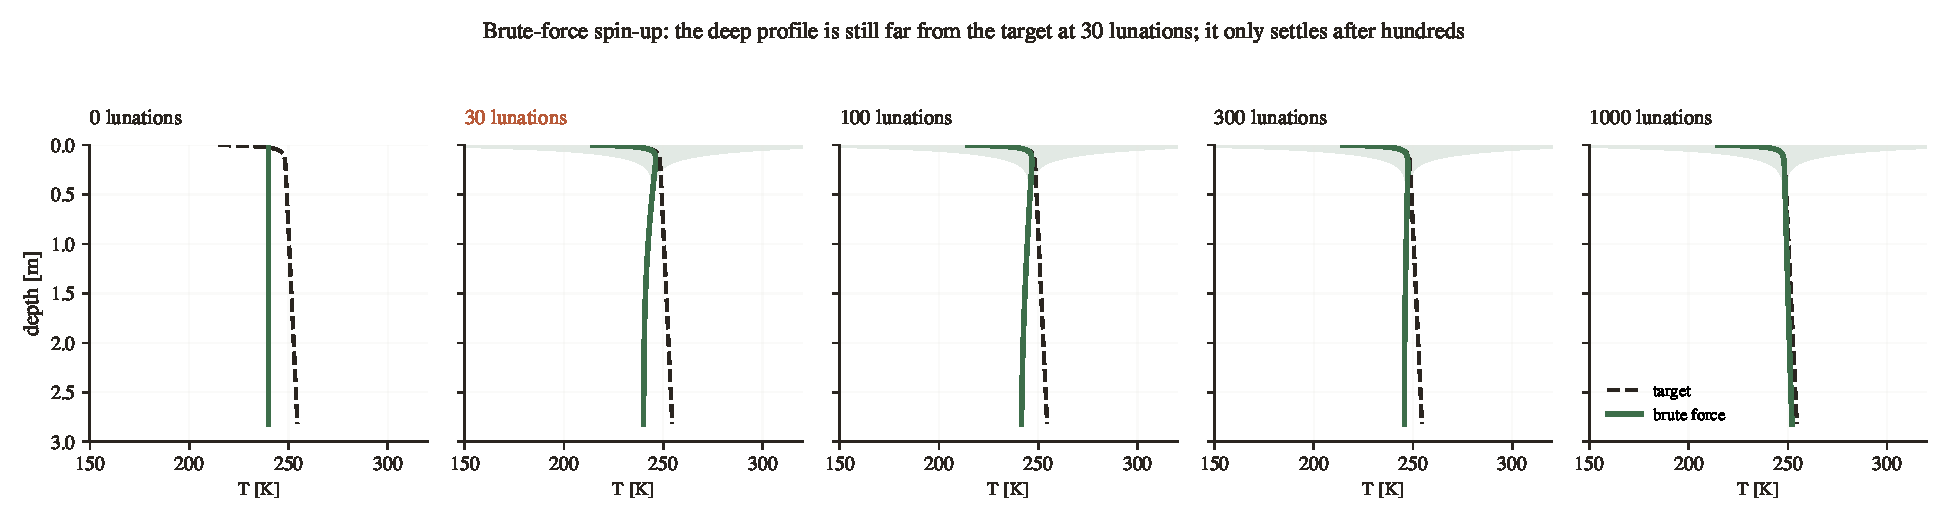
\includegraphics[width=\linewidth]{figures/spinup_filmstrip.pdf}
\caption{Old method (brute force). Green $=$ current profile; dashed $=$ the true
steady state; shaded $=$ daily swing. At 30 lunations only the top has moved; it
takes hundreds of lunations to reach the target.}
\label{fig:film}
\end{figure}

% =====================================================================
\section{The new calculation, in full detail}
% =====================================================================
The new solver keeps the \emph{exact same} time-stepper of \S2.2 --- it does not
change the physics. It only changes \emph{how long} that stepper runs and what
happens between runs. It alternates two moves (\figref{fig:newfilm}; animated in
\code{newmethod.gif}).

\subsection{Step A --- settle the skin}
Run the stepper for a \emph{short} block of $n$ lunations from the current
profile. Because the skin is shallow it equilibrates in a handful of lunations.
Read the cycle-mean ``anchor'' temperature $\Tm(z_0)$ just below the skin.

\subsection{Step B --- reconstruct the deep profile}
From the anchor, integrate Eq.~\eqref{eq:closure} \emph{downward} to set every
deeper cell. The code uses a midpoint (RK2) step (\code{\_reconstruct\_subskin}):
\begin{equation}
q_i = Q_b - u_i,\quad
T_{1/2}=T_i+\tfrac12\frac{q_i}{K(T_i,z_i)}\Delta z,\quad
T_{i+1}=T_i+\frac{q_i}{K(T_{1/2},z_{1/2})}\,\Delta z .
\label{eq:recon}
\end{equation}
This is the move people find surprising: the deep temperatures are not simulated,
they are \emph{computed} by walking down a known slope. With $Q_b=21$\,mW\,m$^{-2}$
and $K\approx9$\,mW\,m$^{-1}$K$^{-1}$ at depth, the slope is $\sim$2.3\,K/m, so
each metre adds $\sim$2.3\,K from the anchor downward (animated in
\code{reconstruct.gif}).

\subsection{The rectification correction \texorpdfstring{$u_i$}{u}}
Near the skin the daily wave is still large, and the cycle-mean of the
\emph{nonlinear} flux is not quite $K(\Tm)\,\partial_z\Tm$; the difference is the
``rectified'' eddy term $u(z)=\langle K\,\partial_zT\rangle-K(\Tm)\,\partial_z\Tm$,
computed exactly from the cycle (\code{\_rectified\_flux}) and subtracted in
Eq.~\eqref{eq:recon}. It is a few percent of $Q_b$ at the anchor and negligible
below $\sim$1\,m, but including it keeps the closure exact.

\subsection{The outer iteration (exact schedule)}
Steps A--B are iterated as a two-stage schedule (\code{solve\_periodic\_equilibrium}):
\begin{center}\small
\begin{tabular}{@{}lcccc@{}}
\toprule
Stage & anchor $z_0$ & inner lunations $n$ & max outer its & stop when drift $<$ \\
\midrule
1 (coarse) & 0.25\,m & 4  & 4  & 0.10\,K \\
2 (fine)   & 0.55\,m & 12 & 20 & 0.005\,K \\
\bottomrule
\end{tabular}
\end{center}
Stage 1 cheaply kills the bulk of the initial-guess error high in the column;
stage 2 anchors below the rectification zone and iterates to tolerance. ``Drift''
is the change in the anchor temperature between successive outer iterations. In
practice this converges in about a dozen outer rounds --- \textbf{$\sim$150
lunations of stepping in total} (the rest of each iteration is the cheap
algebra of Eq.~\eqref{eq:recon}).

\begin{figure}[h]
\centering
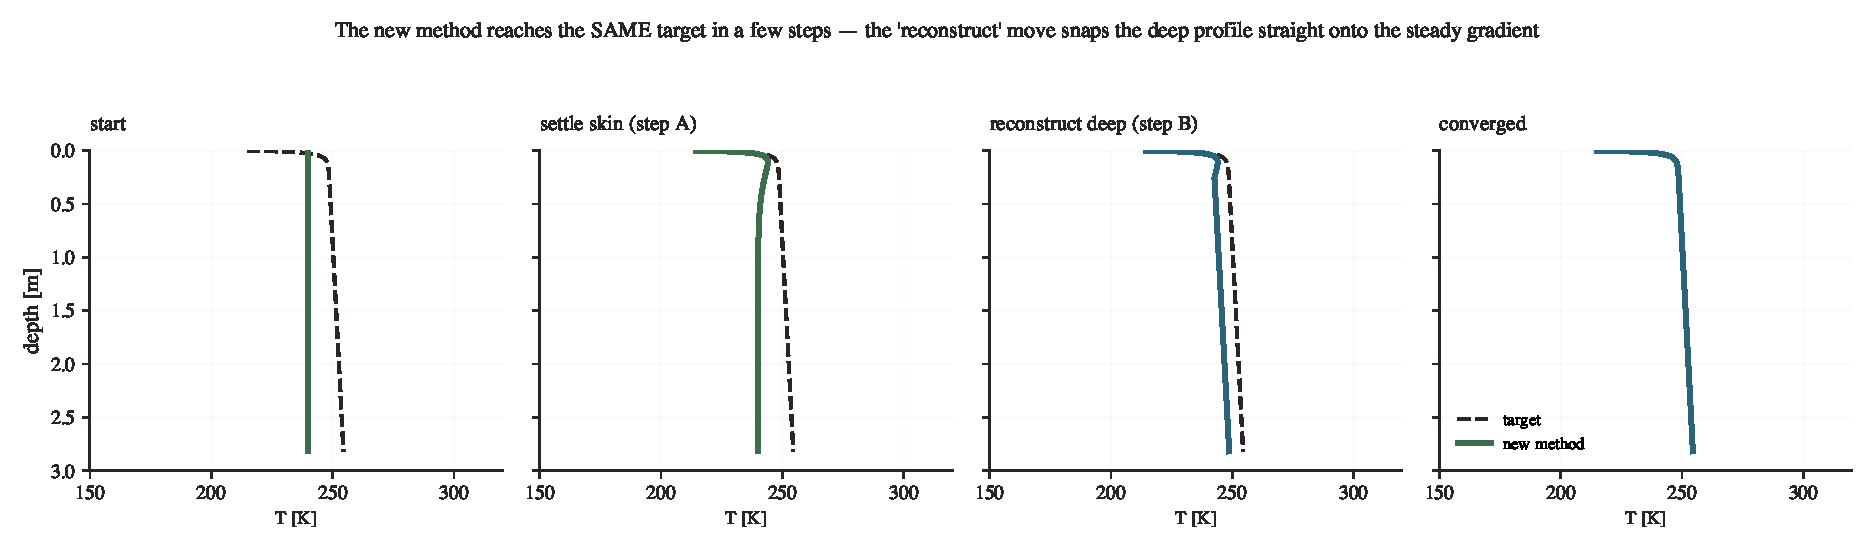
\includegraphics[width=\linewidth]{figures/newmethod_filmstrip.pdf}
\caption{New method. A short spin-up settles the skin (Step A); the reconstruct
move snaps the deep profile onto the steady gradient (Step B); a dozen short
rounds refine it to the target.}
\label{fig:newfilm}
\end{figure}

% =====================================================================
\section{The precise difference between the two calculations}
% =====================================================================
Both run the identical Crank--Nicolson stepper. The difference is entirely in how
the \emph{deep} profile is obtained:

\begin{center}\small
\begin{tabular}{@{}p{4.4cm}p{5.3cm}p{5.3cm}@{}}
\toprule
 & \textbf{Old (brute force)} & \textbf{New (flux-anchored)} \\
\midrule
How the deep profile is set & by waiting for heat to diffuse down over the full $\tau\sim10^3$ lunations & computed directly from $d\Tm/dz=Q_b/K$ (Eq.~\eqref{eq:recon}) after a short skin spin-up \\
Stepping done & $\sim$1000+ lunations in one long run & $\sim$150 lunations, in $\sim$12 short blocks \\
Depends on the initial guess? & yes (if stopped early) & no --- the deep profile is reconstructed each round \\
Convergence test & cycle-to-cycle $\Delta T$ (can give a false positive) & anchor drift $+$ flux closure on $Q_b$ (cannot) \\
Wall time per solve & $\sim$4\,min & $\sim$9\,s \\
\bottomrule
\end{tabular}
\end{center}

\begin{kbox}{forest}
In one sentence: the old method \emph{discovers} the deep gradient $Q_b/K$ slowly
by letting heat diffuse; the new method \emph{writes it down} from energy
conservation and only simulates the fast shallow part. Same physics, same
stepper, same answer --- $\sim$30$\times$ less work.
\end{kbox}

% =====================================================================
\section{How we know the new method is right}
% =====================================================================
Five independent checks, in increasing strength:

\paragraph{(1) Uniqueness (the argument).} Given the anchor value,
Eq.~\eqref{eq:closure} is a first-order ODE with a smooth right-hand side, so it
has exactly one solution below the anchor; the anchor itself is fixed by the
fast surface balance. The periodic steady state is therefore unique. Any method
that satisfies both defining conditions (periodic skin $+$ flux closure) has
found it --- and both methods do.

\paragraph{(2) Self-certification.} Every solve returns two diagnostics: the
anchor \emph{drift} between outer iterations (we require $<0.03$\,K; typically
$\sim$3\,mK) and the \emph{flux closure} $\max|\langle q\rangle-Q_b|/Q_b$ below
the anchor (we require $<2\%$; \figref{fig:cert}). These are exactly the test the
old fixed spin-up could not pass.

\paragraph{(3) Guess-independence.} Starting the new solver from 240\,K and from
260\,K gives sensor-depth temperatures agreeing to $<0.03$\,K. The very symptom
that exposed F1 is now gone.

\paragraph{(4) Brute-force cross-validation (the decisive one).} We take the
\emph{old} method and simply run it far longer. As the lunations increase its
profile marches monotonically onto the new method's answer (\figref{fig:conv}),
and from two different starts it lands on the same curve to tens of mK at
3000 lunations (\figref{fig:overlay}). The two methods agree where it can be
checked directly.

\paragraph{(5) Drift/rectification validation.} A 120-lunation drift test
confirms the neglected higher-order term is $<1\%$ of $Q_b$ below the anchor, so
Eq.~\eqref{eq:recon} closes to the stated tolerance. (Tests:
\code{tests/test\_equilibrium.py}.)

\begin{figure}[h]
\centering
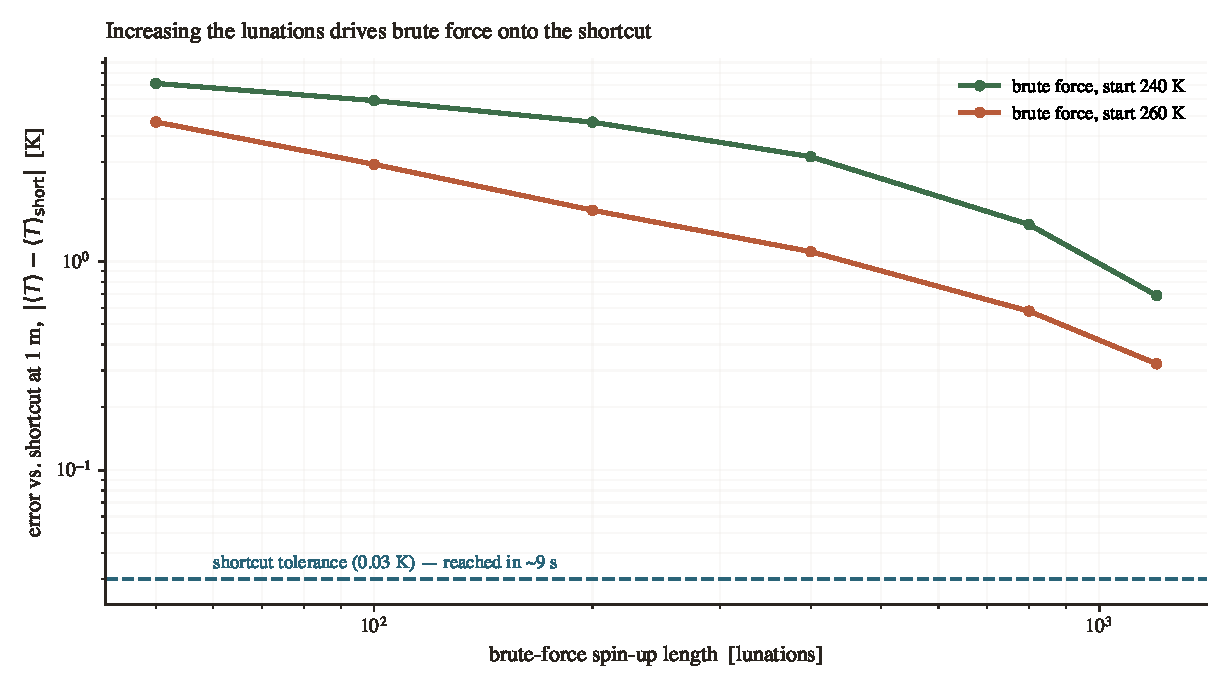
\includegraphics[width=0.70\linewidth]{figures/fig_convergence.pdf}
\caption{Check (4): brute-force error vs.\ the shortcut falls steadily as the
spin-up lengthens; two starts converge to the same place.}
\label{fig:conv}
\end{figure}
\begin{figure}[h]
\centering
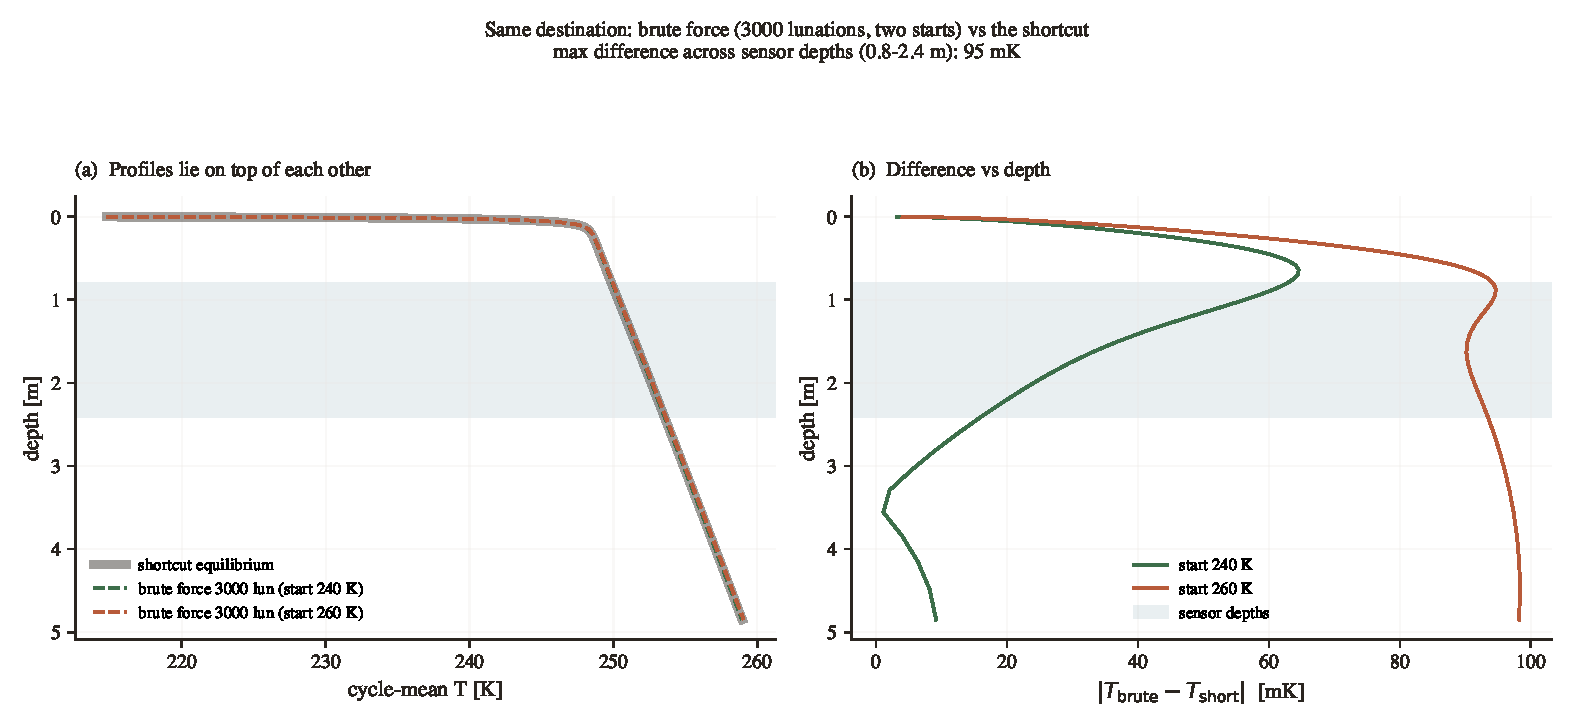
\includegraphics[width=\linewidth]{figures/fig_equilibrium_demo.pdf}
\caption{Brute force to 3000 lunations from 240\,K and 260\,K (dashed) on the
shortcut (solid): indistinguishable; the residual is brute force still finishing.}
\label{fig:overlay}
\end{figure}
\begin{figure}[h]
\centering
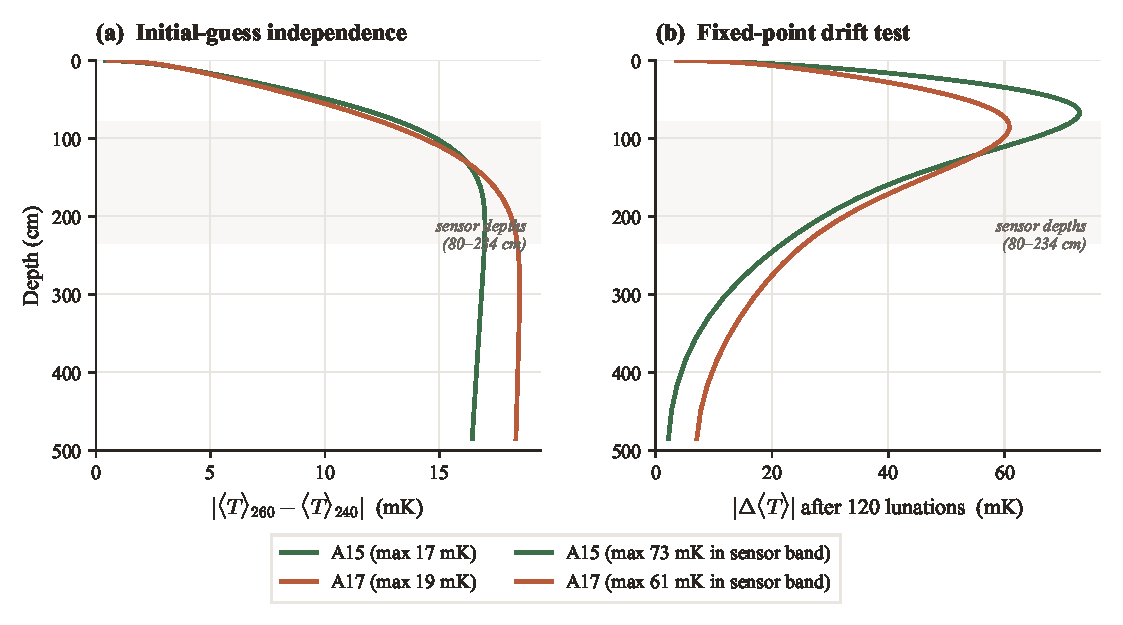
\includegraphics[width=0.80\linewidth]{figures/fig_equilibrium_certification.pdf}
\caption{Check (2): guess-independence and mean-flux closure --- the returned
proof that a solve reached the steady state.}
\label{fig:cert}
\end{figure}

% =====================================================================
\section{Porting to C++}
% =====================================================================
\subsection{Where the time goes}
A solve spends essentially all its time in the inner step (\S2.2), run hundreds
of thousands of times. In the current Python, the tridiagonal \emph{solve}
(\code{\_thomas}) is already JIT-compiled with Numba, but the matrix
\emph{assembly} in \code{\_step} (building $a,b,c,d$ and the face means each step)
is interpreted Python over $\sim$69-element arrays --- many cheap operations per
step, which is exactly the pattern where interpreter overhead dominates. That is
the part a compiled language removes.

\subsection{What to port, what to keep}
The numerics are already isolated in three small, I/O-free modules --- port these:
\begin{itemize}[leftmargin=1.4em,itemsep=1pt]
\item \code{grid.py} --- build the geometric mesh (trivial array construction);
\item \code{solver.py} --- the per-step assembly, the harmonic face means, the
Thomas solve, and the Newton surface balance (\S2.2);
\item \code{equilibrium.py} --- the outer A--B loop and the RK2 reconstruction
(Eq.~\eqref{eq:recon}).
\end{itemize}
Keep \code{config.py} (emit it as JSON so the C++ side reads the same parameters),
and leave the retrieval, statistics, and all plotting in Python calling the fast
core through a thin binding (e.g.\ pybind11). The three-layer code layout
(\figref{fig:arch}) is built for exactly this split.

\begin{figure}[h]
\centering

\includegraphics[width=0.86\linewidth]{figures/fig_architecture.pdf}
\caption{The codebase is layered so the numerics (\code{lunar/}) can be replaced
by a C++ core while the drivers and analysis stay in Python.}
\label{fig:arch}
\end{figure}

\subsection{Expected gain, honestly}
For this tight small-array loop a compiled core typically buys $\sim$10--100$\times$
on the stepping. \textbf{But} much of that is reachable \emph{without} C++:
Numba already compiles \code{\_thomas}, and applying the same \code{@njit} (or a
NumPy vectorisation) to \code{\_step} would capture most of the gain in pure
Python. So C++ is the ceiling, not the only route. The three speed-ups are
independent and multiply: the algorithm (the shortcut, $\sim$30$\times$, already
done) $\times$ compilation (C++/Numba) $\times$ parallelism across independent
solves (the $K_d$ sweep fans over CPU cores). For the present paper, Python plus
the shortcut is already fast enough; C++ pays off when scaling to many DEM pixels
or a mission pipeline that runs the solver millions of times.

\subsection{How to validate the port}
Port bottom-up and regression-test each layer against the Python reference: the
grid arrays must match bit-for-bit; the stepper must reproduce the analytic
constant-coefficient thermal wave (already used in \code{tests/test\_solver.py});
and the full solver must reproduce the committed steady-state profiles and the
\code{drift}/\code{flux\_closure} diagnostics. The existing 37-test suite is the
cross-language regression harness.

% =====================================================================
\section*{How to defend each claim in one line}
% =====================================================================
\begin{itemize}[leftmargin=1.4em,itemsep=2pt]
\item \emph{Why a new method?} A fixed spin-up doesn't reach steady state at
sensor depth, so the initial guess biased $K_d$ (F1).
\item \emph{What it does differently?} It imposes the deep gradient $Q_b/K$
directly instead of waiting $\sim$10$^3$ lunations for diffusion to find it.
\item \emph{How do we know it's right?} It is unique by construction, it
certifies its own convergence, it is guess-independent, and brute force run long
converges onto it.
\item \emph{Faster?} $\sim$9\,s vs $\sim$4\,min per solve; portable to C++ for
another $\sim$10--100$\times$ at scale.
\end{itemize}

\end{document}
